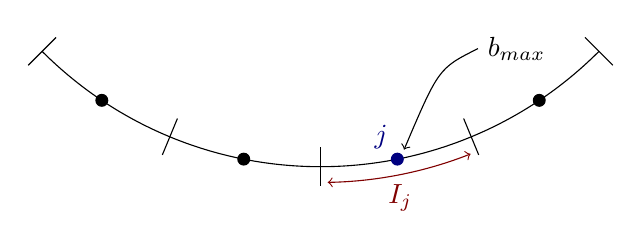
\begin{tikzpicture}
  [scale=5,
  midpoints/.style=blue!50!black,
  intervals/.style=red!50!black]
  \draw (225:1) arc [start angle=225, end angle=315, radius=1];
  \foreach \th in {-2,...,2}
  \draw (270 + 22.5*\th:.95) -- (270 + 22.5*\th:1.05);

  \foreach \th in {236.25,258.75,303.75}
  \filldraw (\th:1) circle [radius=.015];
  
  \filldraw[midpoints] (281.25:1) node [above left] {$\binMidpoint{j}$}
  circle [radius=.015];

  \draw [<->, intervals] (271:1.04) arc [start angle=271, end
  angle=291.5, radius=1.04] node [midway, below] {$I_j$};

  \draw[->] (.4,-.7) node [right,fill=white] {$b_\tn{max}$}
  .. controls (.3, -.75) .. (282.5:.98);
\end{tikzpicture}
